\chapter{Experiments and Testing}
\label{chapter:4}
%% NO PERSONAL FORMS us,we,I
%% quotes use like : ``text''
%% after point,doublepoints and commas there must be a BLANK SPACE

% **************************** Define Graphics Path **************************
\ifpdf
    \graphicspath{{Chapter3/Figs/Raster/}{Chapter3/Figs/PDF/}{Chapter3/Figs/}}
\else
    \graphicspath{{Chapter3/Figs/Vector/}{Chapter3/Figs/}}
\fi

This Chapter is a detailed description about the simulations and experiments carried out on the Invariant Observer.
The first section introduces a survey about the environment of the experiments and their semantic property.
After the first section there comes a short overview  about the simulations with ModelSim.
In the final section there is a detailed description about the test cases and experiments, even something about the performance studies which where
mentioned in subsection~\ref{chapter:3:section:2:sub:3} of Chapter 3 before. \\



\section{Reasoning and Environment of the Experiments}
\label{chapter:4:section:1}
This section should be considered as an answer for the following questions ``Which results do we gain from these experiments?'' and ``How are the experiments done?''. 

\subsection{Reasoning and Meaning}
\label{chapter:4:section:1:subsection:1}
The Invariant Observer will interact in an environment where at least soft real-time, but rather hard real-time conditions will be considered.
Therefore, the correct behaviour has to be shown with regard to the algorithm and the resulting VHDL Implementations.
A good start to show a correct behaviour are simulations, but it should be mentioned that no clear assertions can be made about correct timings of the underlying Design.
This question will be examined in section ``Experiments''.
How the simulations and experiments were executed, and which insights they produced, will be discussed in the next subsection.
After the simulations, to present a first proof about the correct principle of the Invariant Observer, the VHDL Design had to be synthesized on a Hardware.
A FPGA Board was the best solution, besides other possibilities like ASIC's or a Microcontroller. 
An ASIC (Application-specific integrated circuit) is the most performant solution, but that solution is hard-wired and any change of the design is very expensive. 
But it could be considered as the final product implementation.
A Microcontroller would never reach the performance of a FPGA Board and FPGA's are more cost effective and nearly performant like hard-wired solutions. 
Any change of the design can be easily downloaded on a FPGA Board, so it seems logical to use a FPGA as the prototyping platform.
One important part of the experiments was to show the timing boundaries of the Observer Design. 
(e.g. the maximum performance on a FPGA board like the DE2-115, which was used for the experiments).
But other FPGA's with stronger capabilities could reach better performance goals. 
In \cite{RTFMBJ13} for example, several FPGA models were used to reach a more expressive experiment.    
Another part of the experiments was to show the ability of handling any propositional formula $\phi$, 
which is a temporal description of ongoing operations from an observed system. 
The evaluation of $\phi$ takes time, maybe several clock cycles, until the final computation W($\phi$) is finished. 
That circumstance was not exactly tested, but a different approach was introduced to emulate that behaviour. 
A more expressive experiment should be executed if this work will be continued.

The next subsection will explain the detailed investigations of the Invariant Observer through the experiments.   

\subsection{Build-up of Experiments}
\label{chapter:4:section:1:subsection:2}
At the beginning some facts about the Invariant Observer will be repeated, to give a better understanding about the tests that were made.
The Invariant Observer consist of several Observer Stages. 
To cover every clock cycle $e^n$, where a finished computation of a proposition $W(\phi)$ is evaluated, we need at least as many Observer Stages ($m \ge y$), as
the computation (y clock cycles) needs. 
As a reminder, the Observer Stages are not responsible for the computation of the propositions (in contrast to \cite{RTFMBJ13}),
but for the final evaluation of the status of the computation.
So it seems logical to create a signal W($\phi$) which gives, at every clock cycle, a pseudo computation of a proposition $\phi$. 
With that approach, it was easy to show the correct behaviour of the Invariant Observer. 
For example we have m=3 Observer (means theoretically that the computation of $\phi$ needs less than 3 clock cycles), 
and we want to show the invariance of signal W($\phi$), actually the finished computation $W(\phi)$ at every clock cycle, with $\tau = 10$. 
That 3 Observer Stages show whether the signal $W(\phi)$ was invariant 11 clock cycles, the current clock cycle included.
The experiments have been exercised with a plain implementation of a signal $W(\phi)$ and with a more complex implementation of $W(\phi)$, which gives a stronger argument of the correct behaviour.
More about that in the sections ``Experiments'' and ``Simulations''.
These two versions of a simulated input signal for the Observer stages are justified with the fact, 
that the Quartus synthesis tool could create distinct implementations of the Observer Design, because it must match the correct timing behaviours in both cases.   
As a result, the experiments are separated in two parts, as already mentioned in the subsection~\ref{chapter:4:section:1:subsection:1} before, 
but this will be discussed in the section ``Experiments''.   
The next section gives us an insight about the simulations.
%
%A) Reason for tests (behaviour,design improvements,faster design)
%\subsection{}
%B) Test Board , Analyzer ,Versions, Configurations? 
%PF2 -Sampling rate Logic Analyzer

%Top.vhd
%Signalgenerator.vhd

%
%% + SOMETHING ABOUT sIGNALGENERATOR



\section{Simulations}
\label{chapter:4:section:2}
To simulate the VHDL Design of the Observer Stages the simulation tool \textbf{ModelSim (Version 10.1d)} from \textbf{MentorGraphics} was used. 
A testbench, created for simulations in Modelsim, gives a good overview about the intended behaviour of the implemented algorithm and it is useful for debugging and error detection. 
At the beginning, only one Observer Stage was simulated, because it demonstrates the simplest case. 
After error corrections and successful simulations of one Observer Stage, further simulations were proceeded with more Observer Stages. \\
In Figure~\ref{fig:simulation:five} there is illustrated a simulation with m=5 Observer, where every Observer Stage monitors the yellow coloured input signal W($\phi$) for Invariance $\tau=3$. 
The most left column shows the names of the illustrated signals. 
For every Observer (OBS1 to OBS5), signals cycle, $count_p$ and their corresponding outputs (add1 to add5) are shown to overlook their behaviour on the yellow coloured input signal $phi\_s$ (=W($\phi$)). 
Signals cycle and $count_p$ are already described in ~\ref{chapter:sub:2} and ~\ref{chapter:3:section:2:sub:3}, so there is nothing additional. 
Signals add1 to add5 (grey coloured) are the outputs of the different Observer Stages, which are linked together in a binary add operation. 
The result of that operation is illustrated as the red coloured signal $output_s$ which shows the final result of the Invariance Observer. \\
Signal $phi\_s$ is generated by a complex signalgenerator to get a nearly universal test signal. The green coloured signal at the top indicates the system clock which drives the signalgenerator 
and all the Observer Stages at the same time. But the signalgenerator is driven on the rising edge, the Oberver Stages are driven on the falling edge. 
This fact is important to understand one further explanations of the simulation. 
The most important thing that is shown in that illustration is that the Observer Stages activate together the final $output\_s$ exactly $tau + 1$ (with $\tau = 3$) clock cycles after signal phi\_s still holds his active state. 
This case is indicated between these two big vertical lines. 
It shows that the Invariance Observer monitored an Invariance Situation of signal $phi\_s$, according to the behaviour described in Chapter~\ref{chapter:2}. 
That Invariance Situation continues three clock cycles until signal phi\_s goes into a non active state and therefore output\_s. \\
As mentioned before, signal phi\_s changes his state on a rising edge, whereas an Observer Stage checks the state of signal phi\_s on a falling edge. 
This also explains the delayed reaction of the Observer Stages on changes of the input signal as you can see in Figure~\ref{fig:simulation:five}. 
But this handicap could be enhanced by driving the Observers clock a multiple faster. 
The output of the signalgenerator phi\_s is designed in a way to increase the invariance of his active state continuously, so it was reasonable to see how the final red coloured output behaves in comparison with phi\_s. 
To make it clear, signal phi\_s which is created by the signalgenerator only delivers a pseudo input for the Observer Stages which can be understood like as, at every clock cycle, a computation of 
$\phi$ is finished and the result of that computation W($\phi$) is illustrated as true (active state) or false (low state). 
But this also means, also for further simulations and experiments, that the number of Observer Stages in Figure~\ref{fig:observerstages} has no intended meaning. 
There could be less or more than five Observer Stages, the simulation would behave the same. \\  
Finally, it should be discussed how the Observer Stages are initialised. 
The fourth signal from the top enable\_s activates the first Observer Stage which is located at the beginning of an Observer Cascade Chain. 
This principle was already shown in Figure~\ref{fig:observerstages}. 
After one clock cycle the following Observer Stage will be activated by signal en\_1 from the Stage before, and after one clock cycle again signal en\_2 activates the next Observer Stage and so on. 
In Figure~\ref{fig:simulation:five} this behaviour is illustrated at the beginning by signal enable\_s, signals en\_1 till en\_4 and the last output in the cascade by signal next\_obs. \\
A further illustration from another simulation is shown in Appendix~\ref{appendix:2} with m=10 Observer. 
A lot of simulations with different configurations were made, with different numbers of Observer Stages and different Invariance Qualifications. 
Automated Testing was necessary to have a stronger error check in case of changes in the design. 
Assertions as part of the VHDL language were inserted in to the Code to have a possibility to check if the behaviour of the Observer Stages is still the same. 
Modelsim gives also the possibility of scripting, which is very helpful when a lot of simulation parameters have to be handled. \\
The following final section introduces the experiments with a FPGA Board. 


\begin{figure}[]
\centering
%\hspace{3.0cm}
%\vspace{-5cm}
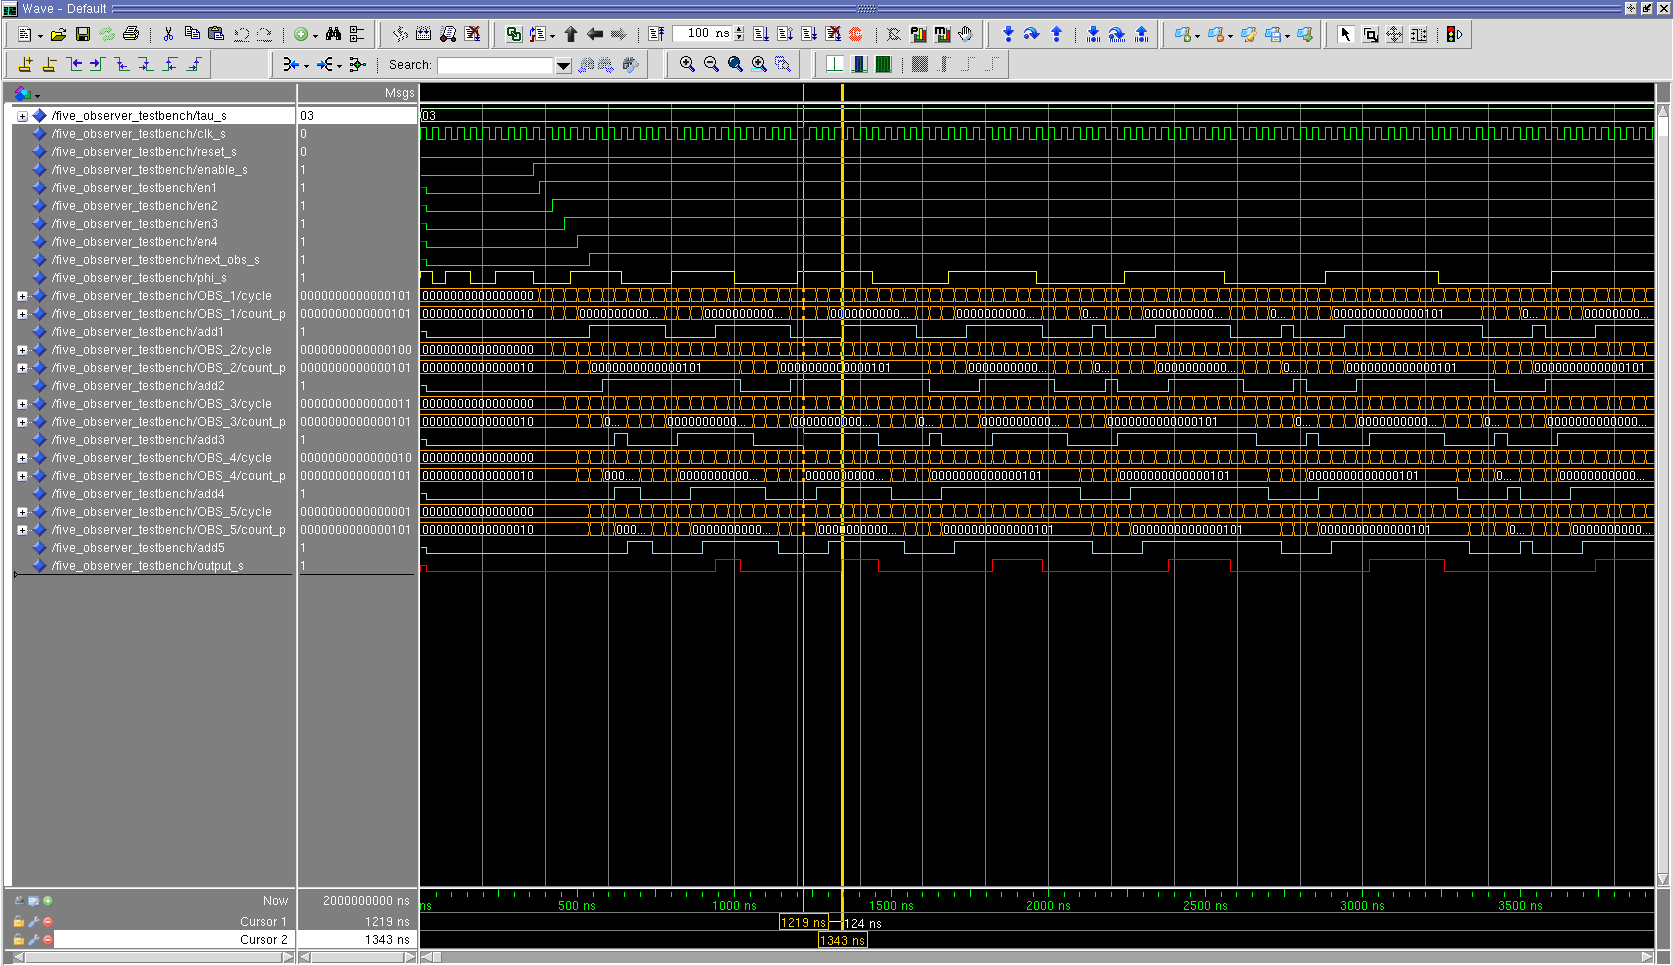
\includegraphics[width=650px,height=300px,angle=-90]{../../pictures/Modelsim/5_Observer_tb_1.png}
%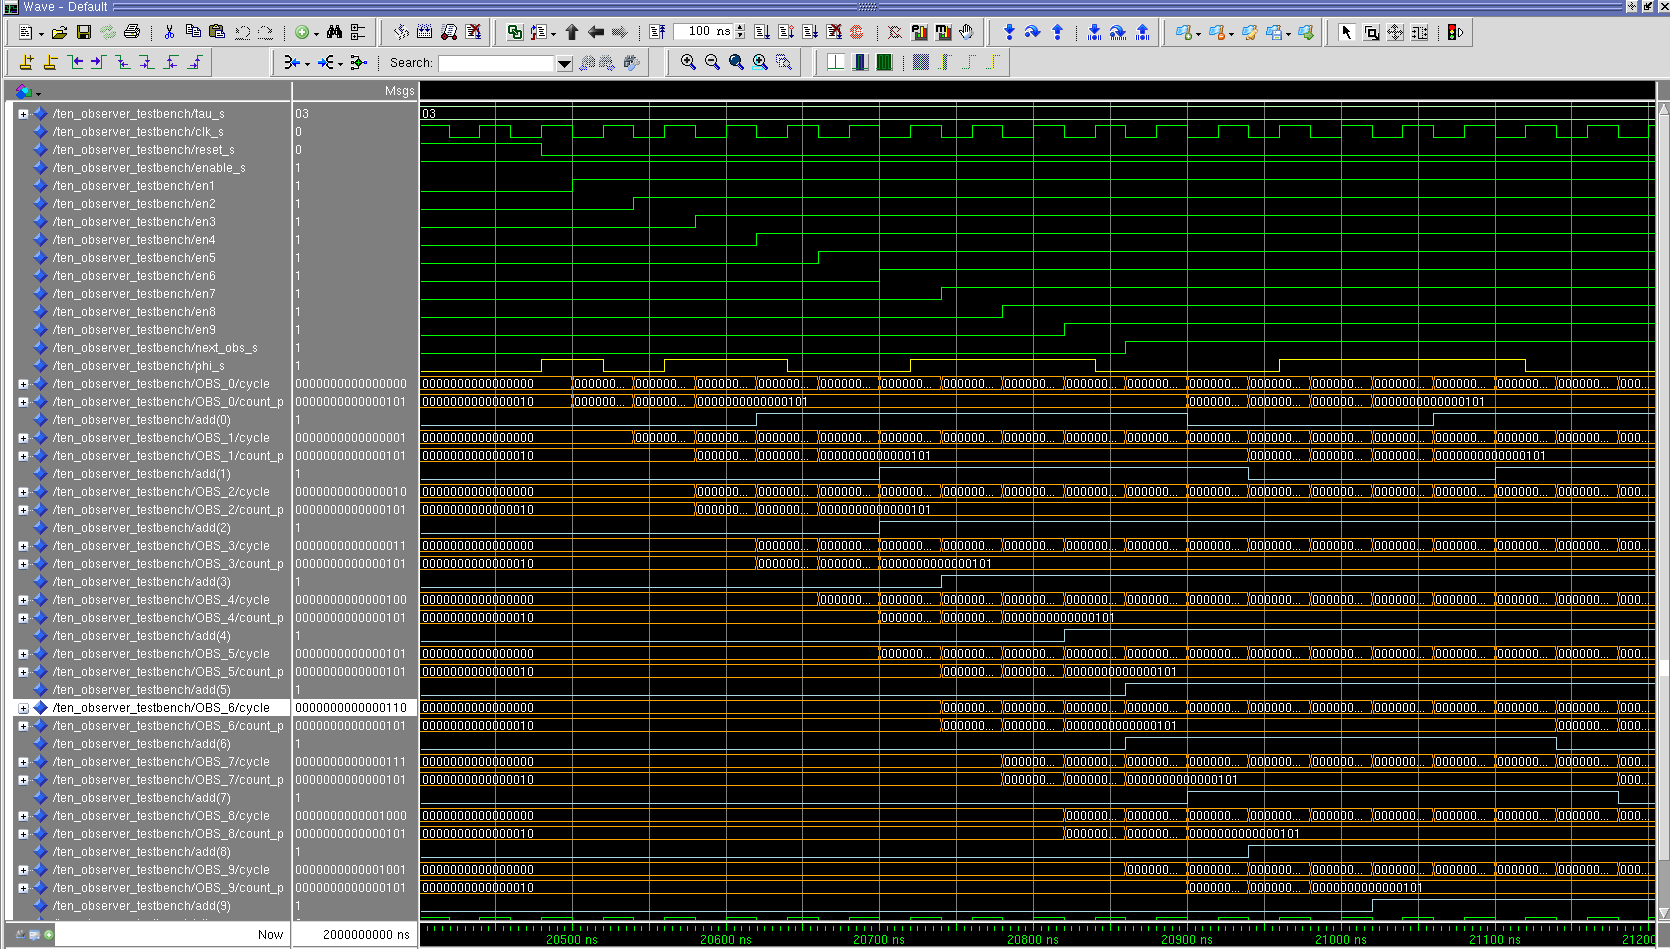
\includegraphics[height]{../../pictures/Modelsim/10_Observer_tb_1.png}
\caption[Modelsim Simulation of 5 Observer]{Illustration of a Simulation with m=5 Observer and Invariance $\tau=3$}
\label{fig:simulation:five}
\end{figure}

\newpage
%C)Simulations
\section{Experiments}
\label{chapter:4:section:3}
This section treats the experiments done for the Invariance Observer Design. 
The main part of the experiments were dedicated for testing the behaviour of the Invariant Observer. 
Other experiments were justified by the reason to figure out the maximum performance of the Observer Design. 
It is decent to present only the edge cases of the experiments, which have reasonable arguments, but that much is clear that a lot of more test cases where exercised. 
For the first, it was important that the correct behaviour of the Invariant Observer was tested and demonstrated on the FPGA Board. 
The correct behaviour of the Invariant Observer Design, synthesized on a DE2-115 FPGA board, will be shown by the following pictures made with the logic analyzer (Agilent 16803A). 
The logic analyzer was used to monitor the output pins \textbf{GPIO(0)} to \textbf{GPIO(34)} from the FPGA Board. 
An example of a TOP VHDL file which embeeds the Invariant Observer Design inside a Test Environment is shown in Appendix~\ref{appendix:1:section:2}. 
A lot of TOP files with different configurations where created, but this one example (~\ref{appendix:source:3} and ~\ref{appendix:source:4}) should only show how the experiments work. 
The output of every Observer Stage is connected to a GPIO output pin, and every of these GPIO pins can be measured and displayed on the logic analyzer. 
The pictures shown for up to 5 Observers (Figure~\ref{fig:logicanalyzer:m5:t10} and Figure~\ref{fig:logicanalyzer:m1:t1}) show only the ouputs from \textbf{GPIO(0)} to \textbf{GPIO(14)} in the left side of every these pictures. 
For 10 Observers, the examples in Figure~\ref{fig:logicanalyzer:m10:t1:1} and Figure~\ref{fig:logicanalyzer:m10:t1:1} illustrate the output pins from \textbf{GPIO(0)} to \textbf{GPIO(31)}. 
For example the first signal \textbf{GPIO(0)} is always the \textbf{reset\_s} signal similar to the arrangement in Figure~\ref{fig:simulation:five}. 
The names of the signals in the following picture are also the same like in the simulation, so it should be clear what the signals in the appropriate line means. 

\subsection{Testing the Behaviour}
\label{chapter:4:section:3:subsection:1}
The experiments in this subsection are realized with a signalgenerator which was build individually to simulate a continuously increasing invariance signal. 
This is only the case, because we want to see the correct behaviour of the Observer Stages indicated by \textbf{add0} to \textbf{addn} and \textbf{final\_output}. 
The signalgenerator and the observer stages are driven with the same input clock of 50Mhz, only for demonstrations. 
An indicated $f_{max}$ means the maximum frequency estimation from the Quartus Tool for the whole design according to the Slow 1200mv 85°C model, which was described in subsection ~\ref{chapter:3:section:2:sub:2}. 
But that will be more considered in the next subsection regarding the performance, whereas this section has no significant arguments regarding the performance of the Observer Stages, 
because $f_{max}$ also depends on the included signalgenerator. 
The pictures in that subsection are very similar to the explanations in Section~\ref{chapter:4:section:2} regarding simulations, so only some few informations will be added.
Every picture contains two clock signals, one for the signalgenerator and one for the Observer Stages, 
this was introduced only for the possibility that the frequency of \textbf{CLK\_OBSERVER} is a multiple of \textbf{CLK\_Generator}, 
but that idea was declined because of some irregular behaviours which will be discussed in the Summary of Chapter~\ref{chapter:5}. 
In principle \textbf{CLK\_Generator} and \textbf{CLK\_OBSERVER} should be the same. 

% Figure~\ref{fig:logicanalyzer:m1:t1}
% Figure~\ref{fig:logicanalyzer:m5:t10}
% Figure~\ref{fig:logicanalyzer:m10:t1:1}
% Figure~\ref{fig:logicanalyzer:m10:t1:2}

The simplest case is what the first picture Figure~\ref{fig:logicanalyzer:m1:t1} shows, is one Observer $m = 1$ and $\tau = 1$ .
Likewise in the simulation explained the vertical lines indicates the start of an active signal phi\_s and the start of it's Invariance Condition.

\begin{figure}[]
\centering
%\hspace{-3.0cm}
%\vspace{-5cm}
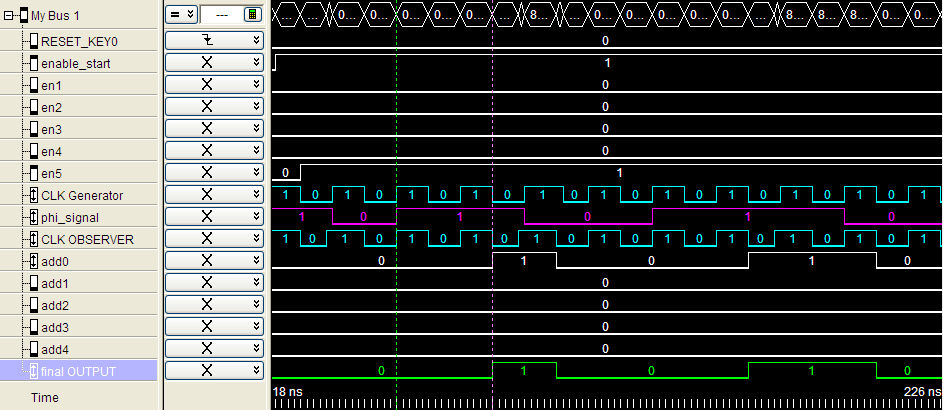
\includegraphics[width=300px,height=150px]{../../pictures/Logicanalyzer/Observer_1_Tau_1.png}
\caption[Logicanalyzer m=1,$\tau=1$]{Illustration from the Logic,only one Observer Stage with m=1,$\tau = 1$}
\label{fig:logicanalyzer:m1:t1}
\end{figure}

\begin{itemize}
 \item $\tau = 1 \;with\; f_{max}=91,41\;Mhz$ (shown in Figure~\ref{fig:logicanalyzer:m1:t1})
 \item $\tau = 10 \;with\; f_{max}=87,61\;Mhz$ 
\end{itemize}

\begin{figure}[]
\centering
%\hspace{-3.0cm}
%\vspace{-5cm}
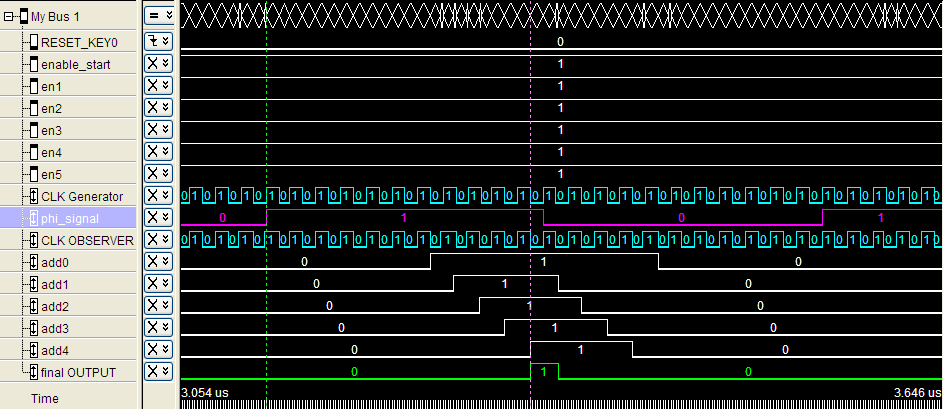
\includegraphics[width=300px,height=150px]{../../pictures/Logicanalyzer/5_Observer_Tau_10.png}
\caption[Logicanalyzer m=5,$\tau = 10$]{Illustration from the Logic analyzer which shows the m=5,$\tau = 10$}
\label{fig:logicanalyzer:m5:t10}
\end{figure}

Figure~\ref{fig:logicanalyzer:m5:t10} shows 5 Observer (m=5) with observing an Invariance of 10 clock cycles\\
Signal \textbf{final\_OUTPUT} is the binary conjunction from \textbf{add0} to \textbf{add4}. 
The vertical lines indicate the beginning of the observation by the Observer Stages (phi\_s in active state) and 
the Invariance Condition $\tau = 10$ fullfilled at the right vertical line. 
If every falling edge of signal \textbf{CLK\_OBSERVER} is counted
between both vertical lines, it should be equal to $\tau + 1 = 11$. 
Same principle should hold for further pictures. 


Figure~\ref{fig:logicanalyzer:m10:t1:1} and Figure~\ref{fig:logicanalyzer:m10:t1:2} show the same experiment (illustration from logic analyzer separated in two pictures) 
with 10 Observer (m=10) which are observing Invariance of $\tau = 1$ on signal phi\_s. 
Figure~\ref{fig:logicanalyzer:m10:t1:2} illustrates the same behaviour like the pictures before. \\
Figure~\ref{fig:logicanalyzer:m10:t1:2} also shows how the Observer Stages are activated, one by one. 
Signal \textbf{enable\_start} shows the start of that start-up sequence, which illustrates the behaviour according to the Algorithm~\ref{alg:observerstage} that 
every Observer Stage turns on the next following Observer Stage after one clock cycle as illustrated by Figure~\ref{fig:observerstages}. \\
\begin{figure}[]
\centering
%\hspace{-3.0cm}
%\vspace{-5cm}
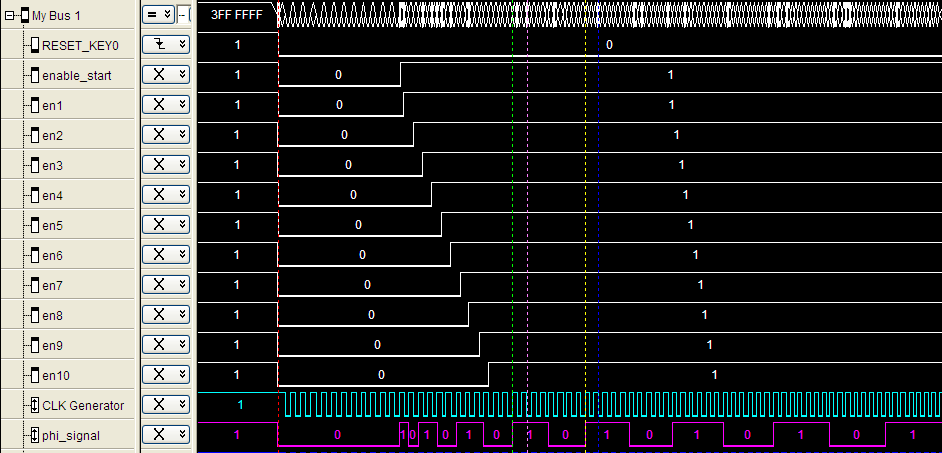
\includegraphics[width=300px,height=150px]{../../pictures/Logicanalyzer/10_Observer_Tau_1_2.png}
\caption[Logicanalyzer m=10,$\tau = 1$]{Illustration from the Logic analyzer which shows the m=10,$\tau = 1$}
\label{fig:logicanalyzer:m10:t1:1}
\end{figure}


\begin{figure}[]
\centering
%\hspace{-3.0cm}
%\vspace{-5cm}
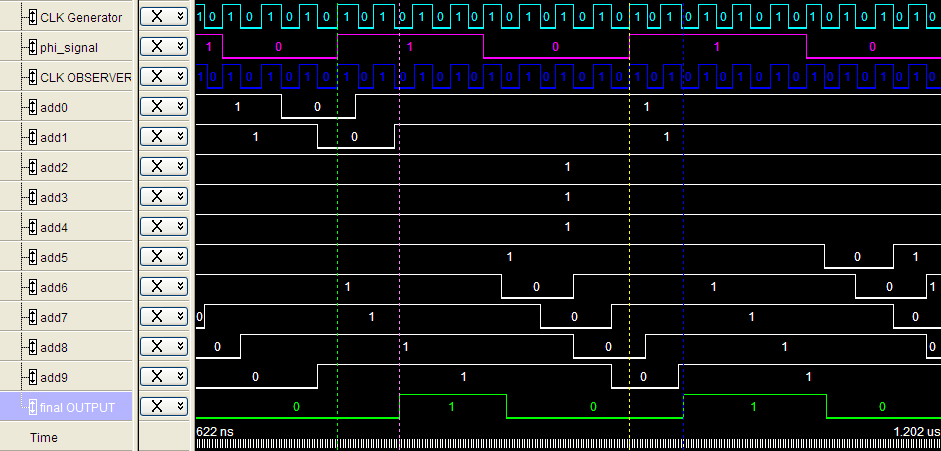
\includegraphics[width=300px,height=150px]{../../pictures/Logicanalyzer/10_Observer_Tau_1_1.png}
\caption[Logicanalyzer m=10,$\tau = 1$]{Illustration from the Logic analyzer which shows the m=10,$\tau = 1$}
\label{fig:logicanalyzer:m10:t1:2}
\end{figure}

The next subsection shows a chain of experiments which could be argued as ``What is the maximum possible clock frequency that can drive the Observer Stages?''

\subsection{Maximum Performance}
\label{chapter:4:section:3:subsection:2}
This subsection discusses the maximum possible performance of the Observer Stage Design under involvement of the limitation by the DE2-115 FPGA Board. 
The following testchain comprise the Invariant Observer Design and a plain Signalgenerator, which only changes the signalvalue of his output at every clock cycle. 
For this experiment it was important that the Quartus II tool take his focus on the Observer circuit, and estimations of the Slow 1200mv 85°C model depends 
only on the Observer Design.
Another modification is that the Phase-Locked Loop (PLL) is used actively, which means that the clock frequency of the Observer Design will be increased in several steps, 
depending on the experiment case. 
At every increase of the input clock frequency, the timing model file (*.sdc) must be updated with the Time Quest Analyzer tool. 
Then depending on the current clock, the number of Observer Stages will be increased, to see the maximum performance for that configuration. 
The maximum range of Invariance $\tau = 255$ is always used, but some experiment cases may have additional tests with another Invariance $\tau$ 
where the differences in the performance can be seen. 
Similar to the previous subsection, $f_{max}$ means the maximum frequency according to the Slow 1200mv 85°C model as a result of the Quartus Timing Model estimation. \\

Legend:\\
(LE is the number of Logic Elements used on the FPGA Board from available 114480LE)
\begin{enumerate}[(1)]
\item Inputfrequency for all Observer Stages: \textbf{50Mhz}
 with plain Signalgenerator
  \begin{enumerate}[a)]
    \item 1 Observer , $\tau = 255$ and $f_{max} = 86,4Mhz$
    \item 10 Observer, $\tau = 255$ and $f_{max} = 101,83Mhz$
    \item 100 Observer, $\tau = 10$ and $f_{max} = 83,81Mhz$  (6718 LE$\sim$6\%)\\
      $\;\;\;\tau = 255$ and $f_{max} = 79,88Mhz$
    \item 300 Observer, $\tau = 255$ and $f_{max} = 74,01Mhz$ 
    \item 1000 Observer, $\tau = 255$ and $f_{max} = 66,00Mhz$ (72514 LE$\sim$63\%)\\\\\\\\
  \end{enumerate}


\item Inputfrequency for all Observer Stages: \textbf{100Mhz}
 with plain Signalgenerator
  \begin{enumerate}[a)]
    \item 1 Observer , $\tau = 255$ and $f_{max} = 96,82Mhz$
    \item 10 Observer, $\tau = 255$ and $f_{max} = 134,99Mhz$
    \item 100 Observer, $\tau = 255$ and $f_{max} = 116,44Mhz$
    \item 1000 Observer, $\tau = 1$ and $f_{max} = 106,09Mhz$ \\
    $\tau = 255$ and $f_{max} = 95,27Mhz$ (72755 LE$\sim$64\%)
  \end{enumerate}


\item Inputfrequency for all Observer Stages: \textbf{200Mhz}
 with plain Signalgenerator
  \begin{enumerate}[a)]
    \item 1 Observer , $\tau = 255$ and $f_{max} = 90,82Mhz$
    \item 10 Observer, $\tau = 255$ and $f_{max} = 139,30Mhz$ (possible \textbf{MAXIMUM})
    \item 100 Observer, $\tau = 255$ and $f_{max} = 114,57Mhz$
    \item 1000 Observer, $\tau = 255$ and $f_{max} = 103,46Mhz$
  \end{enumerate}
\end{enumerate}

In the experiment from (3) case b) the synthesis with the maximum possible performance of the Invariant Observer Design was created by the Quartus Tool.
In Appendix~\ref{appendix:3:section:2} there is an illustration of the RTL View of that design case.
As high the performed input clock is, as well must Quartus sythesize the design to meet the requirements for that frequency. 
This results to the fact that the worst case path time must stay inside the time needed for a clock cycle. 
In all three experiments from (1) to (3) it can be seen that it is not always possible to meet these requirements for an input clock. 
Especially, in the experiments with 200MHZ input clock there is no single case that meets that requirement. 
  
One interesting thing that can be seen in all three experiments (1),(2),(3) is that for case b) with 10 Observers, 
the Quartus tool reach always the maximum performance out of these cases.
1000 Observer occupy nearly 64\% of the capacity of the Logic Elements that a FPGA Board possesses, so that means that the upper bound of possible Observers are close to 1500.
This is the maximum limit of Observers that can be synthesized on the DE2-115 board. 
Other boards with higher capacity are obviously capable to contain more Observers. (e.g. DE4 model series with Stratix IV FPGA cores with up to 820K LE)
Finally, the differences between different values of $\tau$ are not significant as we can see in 1c), 2d), hence the variance keeps inside 10Mhz.

